\documentclass{beamer}

\usepackage[utf8]{inputenc}
\usepackage[T1]{fontenc}
\usepackage{lmodern}
\usepackage[french]{babel}

% Use the default theme and modify the color

\usepackage{amsmath}
\usepackage{xcolor}


\usecolortheme{seahorse}

% Define custom colors
\definecolor{myorange}{RGB}{255, 140, 0}
\definecolor{mywhite}{RGB}{0, 0, 0}

% Set general structure color to orange
\setbeamercolor{structure}{fg=myorange}

% Set frame title background color to orange
\setbeamercolor{frametitle}{bg=myorange, fg=mywhite}

% Customize title page colors
\setbeamercolor{title}{fg=mywhite}
\setbeamercolor{title graphic}{fg=mywhite}
\setbeamercolor{title separator}{fg=mywhite}
\setbeamercolor{subtitle}{fg=mywhite}

\title{Transport optimal, processus poinctuels déterminantaux et le noyau de Bergman}
\date{RECH202}
\author{William Driot}

\usepackage{graphicx}

\begin{document}

% Title page
\begin{frame}

\titlepage

\end{frame}\begin{frame}\frametitle{Processus ponctuels}

    \begin{center}

    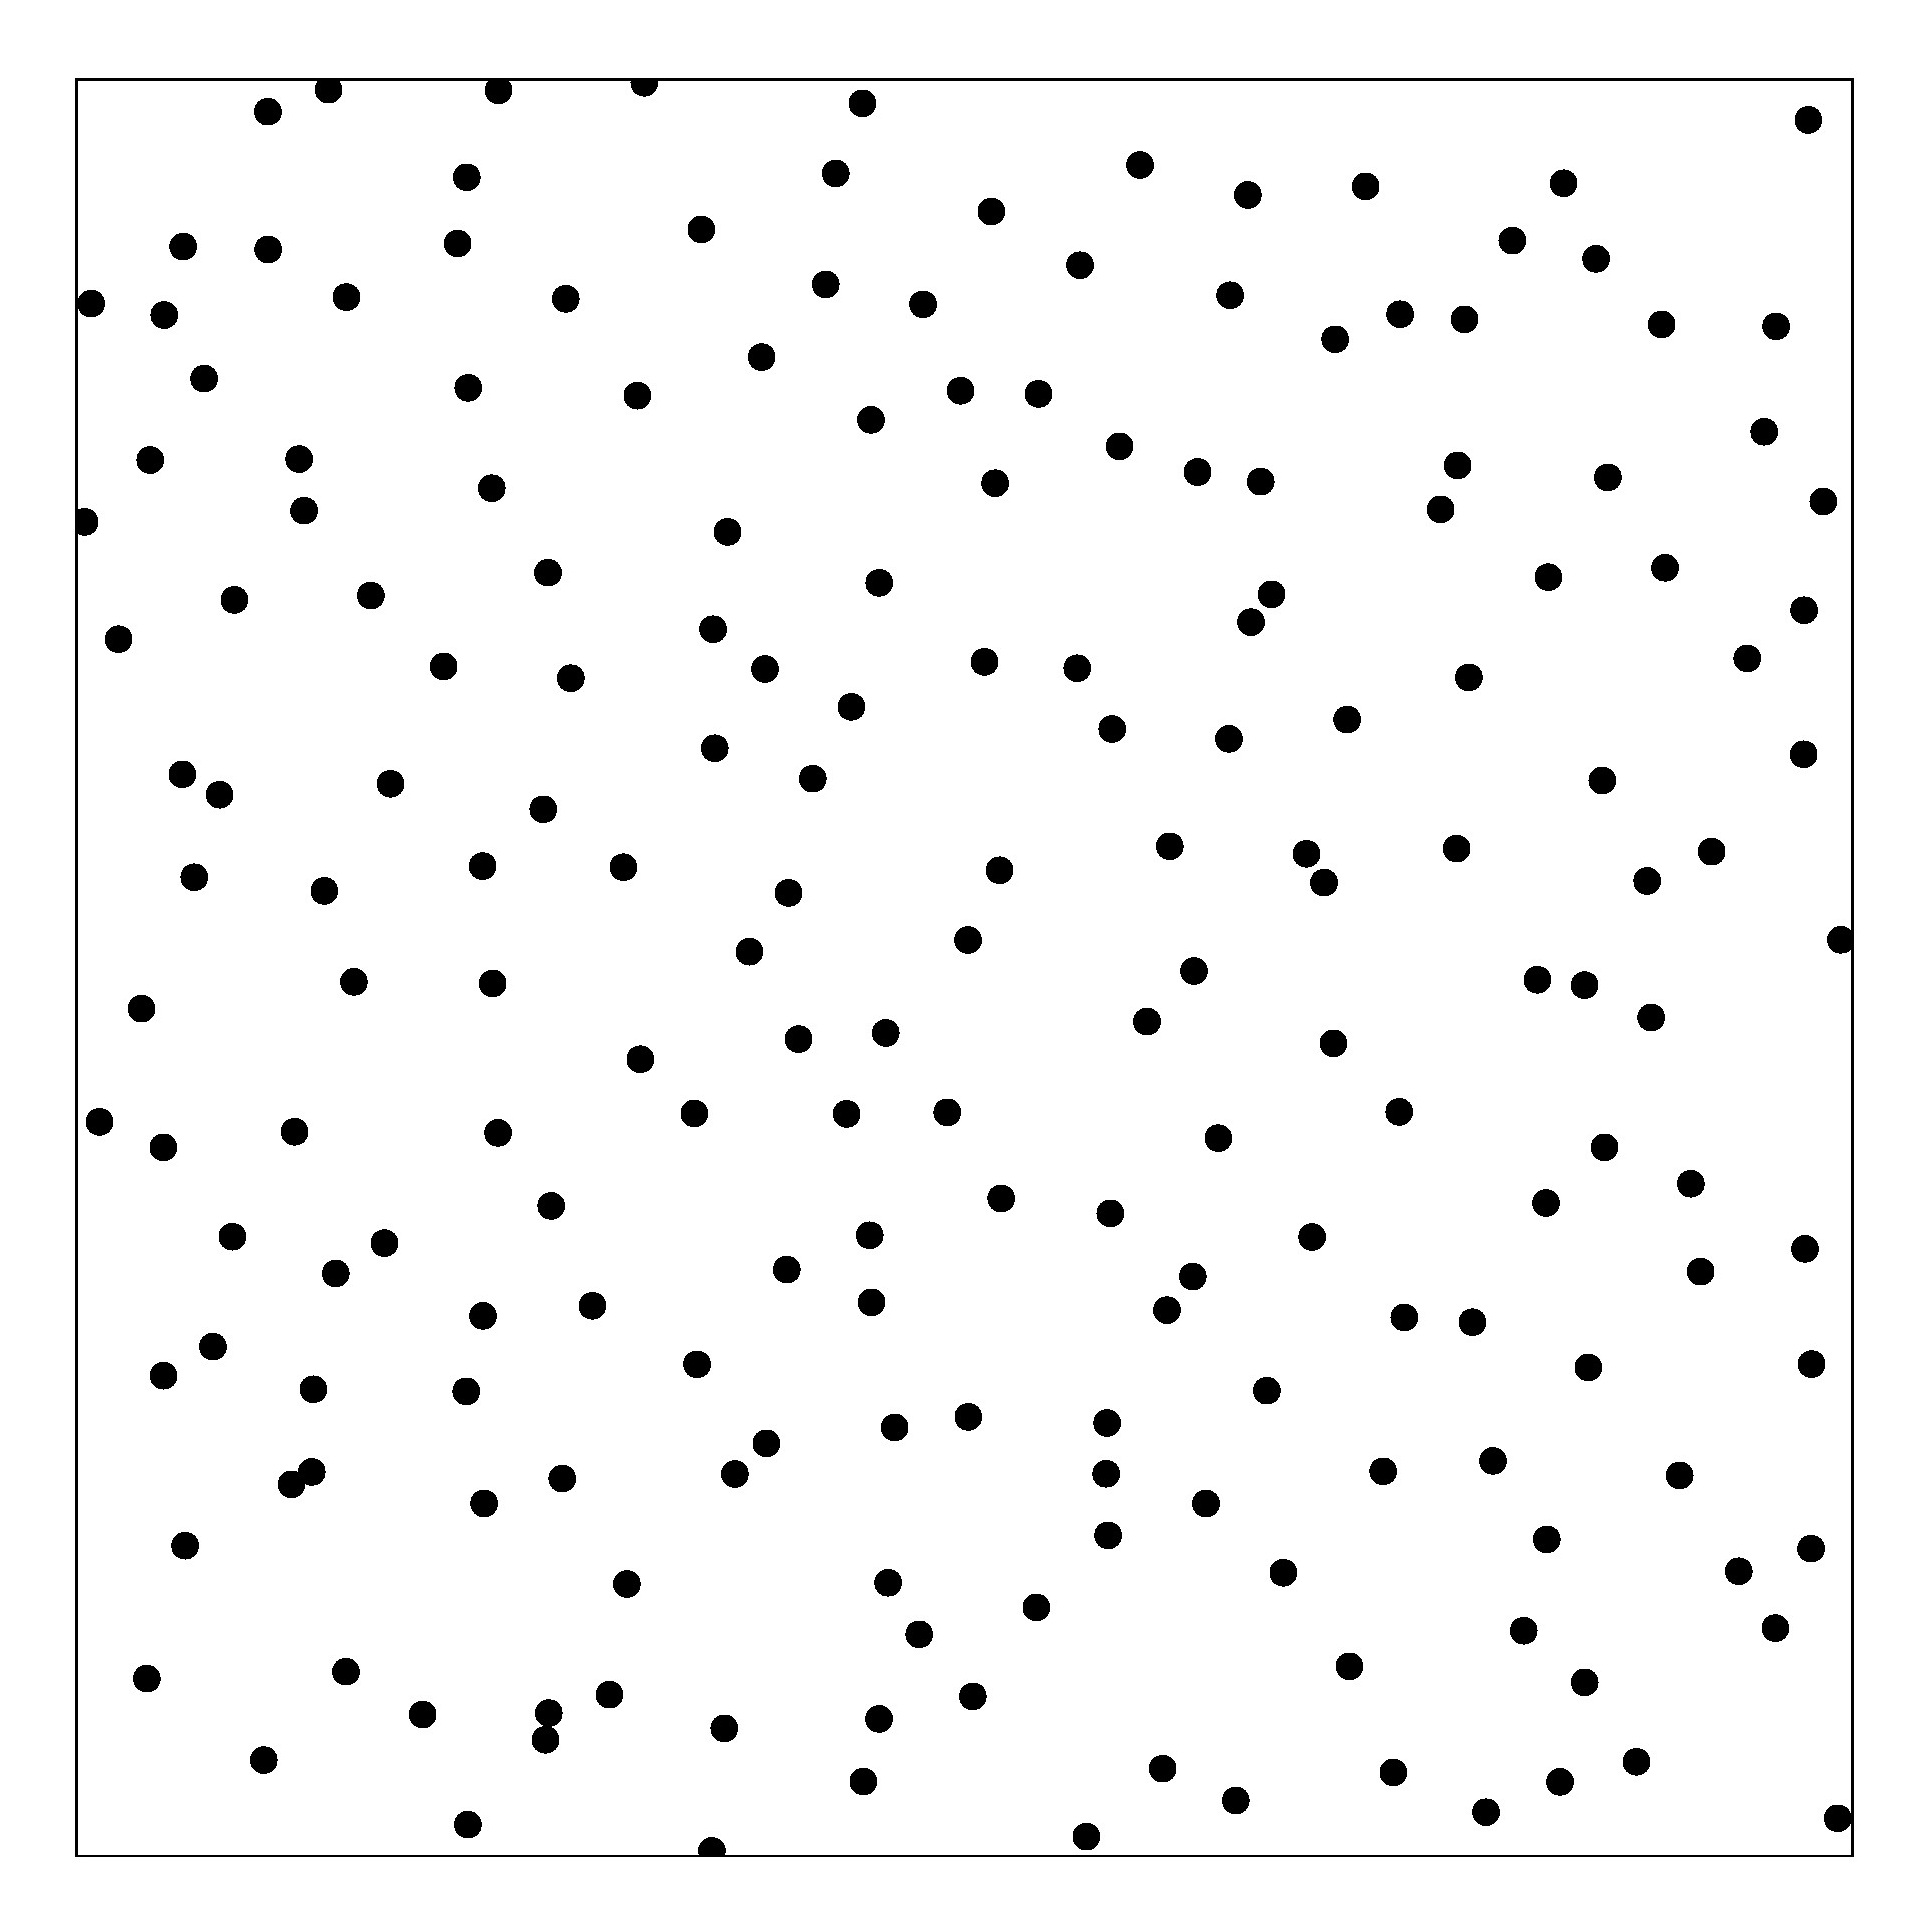
\includegraphics[scale=1]{Points trimmed.jpg}

    
    Un processus ponctuel est une variable aléatoire à valeur dans l'espaces des \og configurations \fg (= parties localement finies, de $ \mathbf C $ par exemple muni de la tribu engendrée par le topologie de la convergence vague).
    \end{center}

\end{frame}\begin{frame}\frametitle{Processus ponctuels déterminantaux}

    \textbf{Définition :}

    Soit $\xi $ un processus ponctuel, $ \lambda $ une mesure de référence sur $E$. $ \xi $  admet $(\rho_n) $ pour fonctions de corrélations si pour toutes parties $A_1,...,A_n$ mesurables \textit{deux à deux disjointes} de $E$, on a $$ \mathbb E \left[ \prod_{k=1}^n \xi(A_k) \right] = \int_{A_1\times ... \times A_n} \rho_n(x_1,...,x_n) \mathrm d \lambda^{\otimes n} $$ Les fonctions de corrélation $ (\rho_n)_{n \in \mathbf N}$ caractérisent la loi d'un processus ponctuel.

    \textbf{Définition :}

    Un processus ponctuel sur $E$ est \textbf{déterminantal} de noyau $k : E^2 \to \mathbf C$ si ses fonctions de corrélation s'écrivent :
    \[
        \rho_n(x_1,...,x_n) = \mathrm{det}(k(x_i,x_j))_{1 \leqslant i,j \leqslant n}
    \]
    où $ k : E^2 \to \mathbf C $ est une fonction $L^2$.

\end{frame}\begin{frame}\frametitle{Écriture de Mercer}

    \textbf{Théorème :} (Mercer)

    \bigskip

    Sur $ (E, \mu) $, soit $ k \in L^2 $ un noyau. On suppose que $k$ est de type positif et que l'opérateur intégral $K$ associé à $k$ est auto-adjoint.

    \bigskip

    Alors les valeurs propres $ \lambda_i $ de l'opérateur intégral $K$ associé à $k$ sont positives, et il existe une base hilbertienne $(\phi_n)_{n\in\mathbf N}$ de $L^2$ formée de vecteurs propres pour $K$, telle que 
    \[
        k(x,y) = \sum_{n \in \mathbf N} \lambda_n \phi_n(x) \overline{\phi_n(y)} 
    \]

\end{frame}\begin{frame}\frametitle{Théorème fondamental}

    \textbf{Théorème :} (fondamental)

    Considérons un DPP de noyau $k$, dont les valeurs propres sont dans $[0,1]$.

    D'après le théorème de Mercer, on peut écrire 
    \[ 
        k(x,y) = \sum_{i \in \mathbf N} \lambda_i \phi_i (x) \overline{\phi_i(y)}
    \] 
    où les $ (\lambda_i)_{i \in I} $ sont les valeurs propres de $K$ dans $[0,1]$.

    \bigskip

    La loi induite par $k$ est la même que celle induite en tirant $ (B_i)_{i \in I} $ des variables aléatoires de Bernoulli indépendantes de paramètres respectifs $ \lambda_i $, puis la loi induite par 
    \[
         k_B(x,y) = \sum_{j \in I} B_j \phi_j(x) \overline{\phi_j(y)}
    \]

\end{frame}\begin{frame}\frametitle{Noyaux de Ginibre et Bergman}

    \bigskip

    Noyau de Ginibre sur $ E = \mathbf C $ : 
    
    $$ k(x,y) = \frac 1 \pi e^{x \overline y} e^{- \frac 1 2 (|x^2| + |y|^2)} = \sum_{n \in \mathbf N} \phi_n(x) \overline{\phi_n(y)}$$

    $$ \phi_n(x) = \frac{1}{\sqrt{\pi n!}} e^{- \frac 1 2 |z|^2} z^n $$

    \bigskip

    Noyau de Bergman sur $ E = \mathcal B(0,1) \subset \mathbf C $ :

    $$ k(x,y) = \frac{1}{\pi(1-x\overline y)^2} = \frac 1 \pi \sum_{k=0}^\infty (k+1)(x \overline y)^k $$

\end{frame}\begin{frame}\frametitle{Simulation}

    \textbf{Problème :} DPPs stationnaires (Ginibre) : les points s'étendent sur $ \mathbf C $ tout entier. 

    \medskip 

    \textbf{Solution :} Restriction à une partie $ \Lambda $, opération mathématique qui construit une variante du DPP pour laquelle il n'y a que des points dans $ \Lambda $.

    \medskip

    \textbf{Problème :} ces DPPs présentent une infinité de points presque sûrement. 

    \medskip

    \textbf{Solution :} Troncation : On considère l'écriture de Mercer $ \sum_{k=0}^{N-1} $ au lieu de $ \sum_{n=0}^\infty $

    \textbf{Question :} Ils sont donc impossibles à simuler stricto-censu. Mais on simule des processus différents ! Ce ne sont plus les mêmes lois !

    \begin{center} $ \rightarrow $ \textbf{Quelle sont les pertes induites par de telles modifications ?}  \end{center}

\end{frame}\begin{frame}\frametitle{1er résultat : Noyau de Bergman restreint}

    \textbf{Théorème.} Soit $\mathcal{B}(0, R)$ le disque de $ \mathbf C $ de centre $0$ et de rayon $R$. On peut (et c'est assez rare pour le souligner) calculer explicitement les valeurs propres et les fonctions propres, et donc la décomposition de Mercer du noyau $k^R(x,y)$ du DPP de Bergman retreint à $\mathcal{B}(0, R)$ :
    \[
    k^R(x,y) = \sum_{n \ge 0} \lambda_n^R \phi_n^R(x) \overline{\phi_n^R(y)},
    \]
    où les valeurs propres sont les 
    \[
    \lambda_k^R = R^{2k+2},
    \]
    et les fonctions propres
    \[
    \phi_k^R : x \mapsto \sqrt{\frac{k+1}{\pi}} \frac{1}{R^{k+1}} x^k.
    \]

    Cet opérateur restreint est à trace donc il présente un nombre \textit{fini} de points p.s. ! 

\end{frame}\begin{frame}\frametitle{Troncation du Bergman projeté}

    \textbf{Rappel :} On ne peut pas simuler un nombre infini de variables aléatoires de Bernoulli. Où s'arrêter alors ?

    \medskip 

    \textbf{Théorème :} Soit
    \[
    N_R := \sum_{n=0}^\infty R^{2n+2} = \frac{R^2}{(1-R)(1+R)}.
    \]
    Soit $\mathfrak{S}^R$ la loi de Bergman restreint au disque compact de rayon $R$ centré en $0$, et $\mathfrak{S}_\alpha^R$ la loi de sa troncation à $\alpha$ points. Si on tronque à $\beta N_R$ points, on a
    \[
        \mathcal{W}_{KR}(\mathfrak{S}^R, \mathfrak{S}_{\beta N_R}^R) \leqslant N_R e^{-2\beta g(R)}
    \]
    où $ g(R) = \frac{R^2}{1+R} $ 

\end{frame}\begin{frame}\frametitle{Distance de Kantorovitch-Rubinstein $ \mathcal W_{KR} $}

    Transport optimal : Sur un espace Polonais $E$, étant donnée une fonction de coût $c : E \times E \to \mathbf R^+ $ sur $E$, et deux probabilités $ \mu $, $ \nu $ sur $E$, minimiser le coût de transport $$ \displaystyle C(\pi) = \int c(x,y) \mathrm d \pi(x,y) $$ sur l'ensemble des couplages $ \pi \in \Pi(\mu,\nu)$ (lois de couples de v.a. de marginales $ \mu, \nu $).

    \textbf{Distance de Wasserstein :} Sur $(E,d)$ polonais, avec $ c_p(x,y) = d(x,y)^p $, $ W_p(\mu, \nu) = \mathcal T_p(\mu, \nu)^{1/p} $ où $ T_p(\mu, \nu) $ désigne le transport optimal entre $ \mu $ et $ \nu $ .

    \begin{center} $\rightarrow $ \textcolor{red}{\textbf{Distances entre lois de probabilités}} \end{center}

    \textbf{Distance de Kantorovitch-Rubinstein : } Pour $ E =$ espace des configurations muni de la distance de variation totale $ d(\xi, \zeta) = | \xi \Delta \zeta| $

    \begin{center} $\rightarrow $ \textcolor{red}{\textbf{Distances entre lois de processus ponctuels!}} \end{center}

\end{frame}\begin{frame}\frametitle{Troncation du Bergman projeté}

    \textbf{Théorème :} Soit
    \[
    N_R := \sum_{n=0}^\infty R^{2n+2} = \frac{R^2}{(1-R)(1+R)}.
    \]
    Soit $\mathfrak{S}^R$ la loi de Bergman restreinte du disque compact de rayon $R$ centré en $0$, et $\mathfrak{S}_\alpha^R$ la loi de sa troncation à $\alpha$ points. Si on tronque à $\beta N_R$ points, on a
    \[
        \mathcal{W}_{KR}(\mathfrak{S}^R, \mathfrak{S}_{\beta N_R}^R) \leqslant N_R e^{-2\beta g(R)}
    \]
    où $ g(R) = \frac{R^2}{1+R} $

    \textbf{Corollaire :}
    \[
    \mathbf{P}(\mathfrak{S}^R \neq \mathfrak{S}_{\beta N_R}^R) \leqslant N_R e^{-2\beta \frac{R^2}{1+R}}.
    \]

    Autrement dit, tronquer au delà de $ N_R $ induit des distances (de Wasserstein) exponentiellement faibles entre les lois des processus. Donc $ N_R $ est un bon choix.

\end{frame}\begin{frame}\frametitle{Convergence en Wasserstein}

    \textbf{Question :} Notre borne ne tend pas vers $0$ quand $ R \to 1^-$. Mais a-t-on quand même 
    \[ 
        \mathcal W_{KR} ( \mathfrak S^R, \mathfrak S) \xrightarrow[R \to 1^-]{} 0
    \] ?

    \textbf{Autre question :} Tronquer à l'espérance ? Mais, par définition, une v.a. peut dépasser son espérance, non ?

    \textbf{Autre question :} Peut-on

    \textbf{Théorème :} (Decreusefond, Moroz, 2021)
    
    Soit $R > 0$. On tronque le Ginibre projeté à $ N_R = (R+c)^2 $ points. Soient $ \xi^R $ et $ \xi^R_{N_R} $ des DPPs ayant ces lois (projeté / projeté et tronqué). Alors
    \[
         \mathcal W_{KR}(\xi^R, \xi^R_{N_R}) \leqslant \sqrt{\frac{2}{\pi}} R e^{-c^2}
    \]

    \textbf{Observation :} En fait, il s'avère que $ R^2 $ n'est autre que l'espérance du nombre de points !

    \begin{center}

    $ \rightarrow $ ce résultat majore la \textbf{déviation} du nombre de points autour de son espérance. 

    Le nôtre aussi, et en est un analogue pour le processus de Bergman.

    \end{center}

\end{frame}\begin{frame}\frametitle{Tronquer à l'espérance}

    \textbf{Théorème :} (Decreusefond, Moroz, 2021)
    
    Soit $R > 0$. On tronque le Ginibre projeté à $ N_R = (R+c)^2 $ points. Soient $ \xi^R $ et $ \xi^R_{N_R} $ des DPPs ayant ces lois (projeté / projeté et tronqué). Alors
    \[
         \mathcal W_{KR}(\xi^R, \xi^R_{N_R}) \leqslant \sqrt{\frac{2}{\pi}} R e^{-c^2}
    \]

    \textbf{Observation :} En fait, il s'avère que $ R^2 $ n'est autre que l'espérance du nombre de points !

    \begin{center}

    $ \rightarrow $ ce résultat majore la \textbf{déviation} du nombre de points autour de son espérance. 

    Le nôtre aussi, et en est un analogue pour le processus de Bergman.

    \end{center}

\end{frame}\begin{frame}\frametitle{Distances de Wasserstein}

    Sur un espace $(E,d)$ polonais, avec $ c_p(x,y) = d(x,y)^p $

    En notant $$ \mathcal T_p(\mu, \nu) = \inf_{\pi \in \Pi(\mu,\nu)} = \iint c_p(x,y) \mathrm d \pi(x,y) = \iint d(x,y)^p \mathrm d \pi(x,y) $$ 

    le coût de transport optimal, $$ W_p(\mu, \nu) = \mathcal T_p(\mu, \nu)^{1/p} $$

    définit une distance sur l'ensemble $ \mathcal P_p(X) $ des mesures boréliennes admettant un moment d'ordre $p$ (= $ \exists x_0, \int d(x_0,x)^p \mathrm d \mu(x) < \infty $)

\end{frame}\begin{frame}\frametitle{Distances de Wasserstein entre DPPs}

    \textbf{Définition :}

    La distance de Kantorovich-Rubinstein est la distance de Wasserstein-1 pour la distance $$ d(\xi, \zeta) = | \xi \Delta \zeta | $$ sur l'espace des configurations. $$ \mathcal W_{KR}(\mu, \nu) = \inf_{\pi \in \Pi(\xi, \zeta)} \mathbb E_\pi(|\xi \Delta \zeta|) $$ 

    \bigskip

    \textbf{Théorème :} (Decreusefond, Moroz, 2021)
    
    Soit $R > 0$. On tronque le Ginibre projeté à $ N_R = (R+c)^2 $ points. Soient $ \xi^R $ et $ \xi^R_{N_R} $ des DPPs ayant ces lois (projeté / projeté et tronqué)

    Alors $$ \mathcal W_{KR}(\xi^R, \xi^R_{N_R}) \leqslant \sqrt{\frac{2}{\pi}} R e^{-c^2} $$

\end{frame}\begin{frame}\frametitle{Perspectives}

    \textbf{Théorème :} (Decreusefond, Moroz, 2021)
    
    Soit $R > 0$. On tronque le Ginibre projeté à $ N_R = (R+c)^2 $ points. Soient $ \xi^R $ et $ \xi^R_{N_R} $ des DPPs ayant ces lois.

    Alors $$ \mathcal W_{KR}(\xi^R, \xi^R_{N_R}) \leqslant \sqrt{\frac{2}{\pi}} R e^{-c^2} $$

    \bigskip $\rightarrow$ Prolongement de ce résultat à d'autres DPPs ? (Noyau de Bergman)

% \end{frame}\begin{frame}\frametitle{Un conjecture en transport optimal ?}

%     \textbf{Conjecture :}

%     \bigskip

%     Soit $E = \mathbf R^n $ muni de sa tribu borélienne. Soient $A,B$ deux parties mesurables de $E$, ayant peut-être une régularité à préciser (ouverts...). Soient $ \mu_A, \mu_B$ les mesures uniformes sur $A,B$ respectivement.

%     Soit $ T : \mathbf R^n \to \mathbf R^n $ une application qui soit un $\mathcal C^1$-difféomorphisme de $\mathbf R^n$. On note $ J_T $ sa Jacobienne.

%     \bigskip

%     Alors $T$ est un application de transport de $ \mu $ vers $ \nu $ ($ \mu_B = T_{\# \mu_A} $) si et seulement si :

%     (1) $T(A) = B$ \qquad     (2) $ |\mathrm{det} (J_T(x))| = 1 $ pour tout $x \in A$.

%     \bigskip

%     $T$ étant un $\mathcal C^1$-difféomorphisme de $ \mathbf R^n $, ces condition équivalent à

%     (1) $A = T^{-1}(B)$ \qquad     (2) $ |\mathrm{det} (J_{T^{-1}}(y))| = 1 $ pour tout $y \in B$.

\end{frame}\begin{frame}\frametitle{Un conjecture en transport optimal ?}

    \textbf{Conjecture :}

    \bigskip

    Soient $A,B \subset \mathbf R^n $ mesurables (ouverts...), $ \mu_A, \mu_B$ les mesures uniformes sur $A,B$.

    Soit $ T : \mathbf R^n \to \mathbf R^n $ un $\mathcal C^1$-difféomorphisme de $\mathbf R^n$. On note $ J_T $ sa Jacobienne.

    \bigskip

    Alors $T$ est un application de transport de $ \mu_A $ vers $ \mu_B $ ($ \mu_B = T_{\# \mu_A} $) ssi :

    \bigskip

    (1) $T(A) = B$ \qquad     (2) $ \forall x \in A, |\mathrm{det} (J_T(x))| = \lambda(B) / \lambda(A)  $ 

    \bigskip

    ou encore 

    \bigskip

    (1) $A = T^{-1}(B)$ \qquad     (2) $ \forall y \in B,  |\mathrm{det} (J_{T^{-1}}(y))| =  \lambda(A) / \lambda(B)$


\end{frame}\begin{frame}\frametitle{Généralisation ?}

    \textbf{Conjecture ?}

    Soient $\mu, \nu $ deux mesures de densités $ f,g $ (continues ?) par rapport à la mesure $ \lambda $ de Lebesgue sur $ \mathbf R^n $.

    Soit $ T : \mathbf R^n \to \mathbf R^n $ un $\mathcal C^1$-difféomorphisme, $ J_T $ sa Jacobienne. $T$ est une application de transport de $ \mu $ vers $ \nu $ ($ \nu = T_{\# \mu } $) ssi :

    (1) $T(A) = B$ 

    (2) $ \displaystyle \left|\mathrm{det} (J_T(x))\right| = \frac{f(x)}{g(T(x))}  $ pour ($\lambda$-presque) tout $x \in A$.

    \bigskip

    Ce qui équivaut à

    (1) $A = T^{-1}(B)$ 

    (2) $ \displaystyle \left|\mathrm{det} (J_{T^{-1}}(y)) \right| = \frac{f(T^{-1}(y))}{g(y)} $ pour ($\lambda$-presque) tout $y \in B$.

    \bigskip

    Si $f$,$g$ sont continues sur $A$ et $B$ : $\iff$ la même chose sans "($\lambda$-presque)"\,.
    
    Pour $f = \mathbf 1_A / \lambda(A) $ et $ g = \mathbf 1_B / \lambda(B) $, on retrouve le cas précédent.


\end{frame}\end{document}